\documentclass[landscape]{slides}

% Definition of the footer
% Institution logo
\def\eniclogo{
\includegraphics[height=2EM]{enic.eps}}
\def\miirelogo{
\includegraphics[height=1EM]{logomiire.eps}}
\def\poesialogo{
\includegraphics[height=1.5EM]{poesiaicon.eps}}
\def\footer{\em{zheng@enic.fr\hfill 10-06-2003}}

%\usepackage[ignore]{advi-slides}
\usepackage{advi-slides}

\advibg[global]{color=[named]{NavyBlue}}
\advitransition[global]{slide}

\setlength{\parskip}{1ex plus 0.5ex minus 0.2ex}

\begin{document}

\firstslide{\Large Statistical Models for Skin Detection}

\begin{center}

\eniclogo \hspace{2em} \miirelogo 

{\bf \em Huicheng ZHENG} \\
zheng@enic.fr \\[0.5em]

{\bf \em POESIA PROJECT(2117/27572)} \\
{\bf \em www.poesia-filter.org} \\
\poesialogo

June $10$ 2003

\end{center}

\newslide{Skin Detection}

{\bf \em Detecting human skin pixels from an image}

\hspace*{3em}
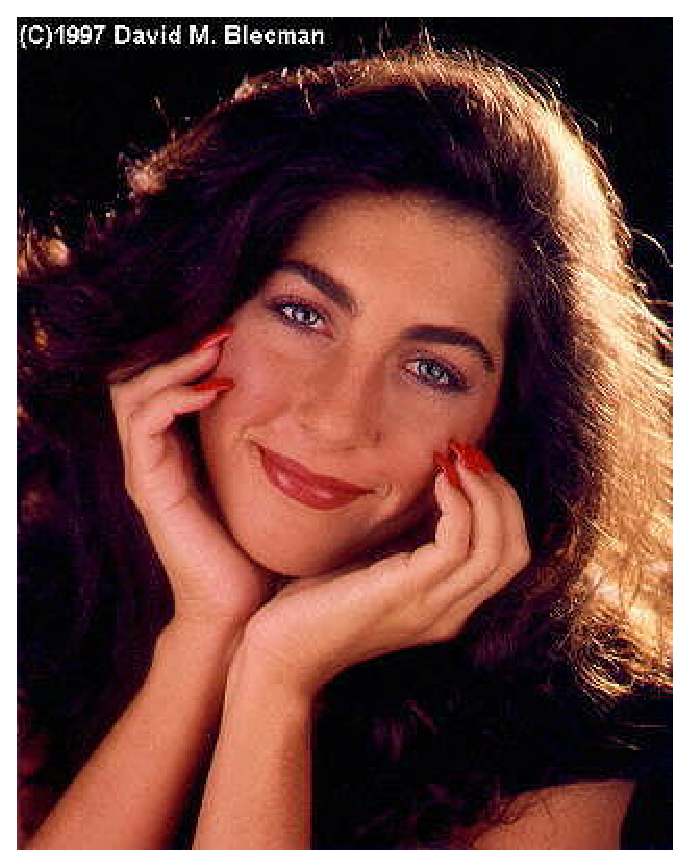
\includegraphics[width=6em]{labelimage.eps} \hfill
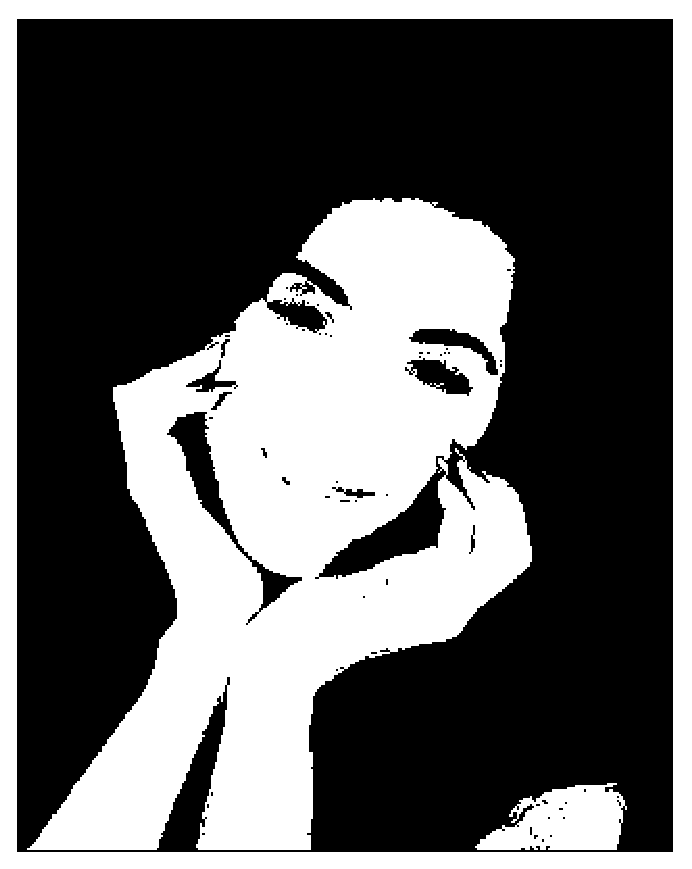
\includegraphics[width=6em]{labelmask.eps} \hspace*{3em}

Applications: face detection, searching and filtering image,\ldots

{\bf \em {Questions}}

1. Variation in skin colors 

\newcommand{\includewhiteeps}[2][]%
 {\epswhite{\includegraphics[#1]{#2}} \epstransparent}
\includewhiteeps[height=5em]{skincolor01.eps} \hfill
\includewhiteeps[height=5em]{skincolor02.eps} \hfill
\includewhiteeps[height=5em]{skincolor03.eps} \hfill
\includewhiteeps[height=5em]{skincolor04.eps} \hfill
\includewhiteeps[height=5em]{skincolor05.eps} \\[1.5em]
\includewhiteeps[height=5em]{skincolor06.eps} \hfill
\includewhiteeps[height=5em]{skincolor07.eps} \hfill
\includewhiteeps[height=5em]{skincolor08.eps} \hfill
\includewhiteeps[height=5em]{skincolor09.eps} \hfill
\includewhiteeps[height=5em]{skincolor10.eps}

2. Variation of the capturing conditions

Illumination conditions, camera, compression loss, noise,\ldots

\includewhiteeps[height=5em]{varvague01.eps} \hfill
\includewhiteeps[height=5em]{varvague02.eps} \hfill
\includewhiteeps[height=5em]{varsaturation01.eps} \hfill
\includewhiteeps[height=5em]{varsaturation02.eps} 

\includewhiteeps[height=5em]{varsatubias.eps} \hfill
\includewhiteeps[height=5em]{varchronbias.eps} \hfill
\includewhiteeps[height=5em]{varmask.eps} \hfill
\includewhiteeps[height=5em]{varbackground.eps}

\newslide{The end}

\begin{center}

\eniclogo \hspace{2em} \miirelogo 

{\bf \em Huicheng ZHENG} \\
zheng@enic.fr \\[0.5em]

{\bf \em POESIA PROJECT(2117/27572)} \\
{\bf \em www.poesia-filter.org} \\
\poesialogo

June $10$ 2003

\end{center}

\end{document}
